\documentclass[10pt]{beamer}

\usetheme[progressbar=frametitle]{metropolis}
\usepackage{appendixnumberbeamer}

\usepackage{booktabs}
\usepackage[scale=2]{ccicons}

\usepackage{pgfplots}
\usepgfplotslibrary{dateplot}

\usepackage{xspace}
\newcommand{\themename}{\textbf{\textsc{metropolis}}\xspace}

\title{Output Dynamics in Real-Business-Cycle Models}
\subtitle{Timothy Cogley and James M. Nason}
\date{\today}

\author{Zixuan, Huixin, Rémi}
\institute{M2 ETE Macroeconomics 2}
% \titlegraphic{%
%     
\includegraphics[width=.3\textwidth]{TSE_Logo_2019.png}\hfill
% }

% \makeatletter
% \setbeamertemplate{title page}{
%   \begin{minipage}[b][\paperheight]{\textwidth}
%     \vfill%
%     \ifx\inserttitle\@empty\else\usebeamertemplate*{title}\fi
%     \ifx\insertsubtitle\@empty\else\usebeamertemplate*{subtitle}\fi
%     \usebeamertemplate*{title separator}
%     \ifx\beamer@shortauthor\@empty\else\usebeamertemplate*{author}\fi
%     \ifx\insertdate\@empty\else\usebeamertemplate*{date}\fi
%     \ifx\insertinstitute\@empty\else\usebeamertemplate*{institute}\fi
%     \vfill
%     \ifx\inserttitlegraphic\@empty\else\inserttitlegraphic\fi
%     \vspace*{1cm}
%   \end{minipage}
% }
% \makeatother

\begin{document}

\maketitle

\begin{frame}{Table of contents}
  \setbeamertemplate{section in toc}[sections numbered]
  \tableofcontents%[hideallsubsections]
\end{frame}

\section{Introduction}

\begin{frame}{Introduction}
    \textit{Are RBC models consistent with output dynamics stylized facts?}\\
    $\Rightarrow$ Compare \alert{output dynamics} in the theoretical RBC model literature and \alert{stylized facts} in the output dynamics analysis\\[1em]  

    \begin{itemize}
        \item Stylized fact \#1: \alert{Autocorrelation} for output growth
        \begin{itemize}
            \item Short horizons: \textbf{Positive and significant} 
            \item Long horizons: \textbf{Negative but insignificant} 
        \end{itemize}
    \end{itemize} 
    \begin{figure}
        \centering
        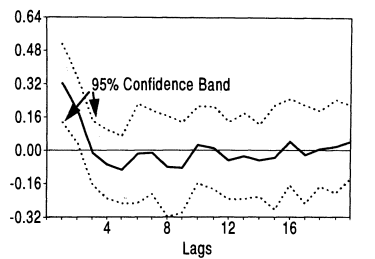
\includegraphics[width=5cm]{sf1.png}
        \caption{Autocorrelation function for output growth}
    \end{figure}
\end{frame}

\begin{frame}
    \begin{itemize}
    \setlength\itemsep{1em}
        \item Stylized fact \#2: \alert{Impulse-response functions} of output
        \begin{itemize}
            \item \textbf{Permanent shock} $\varepsilon_z$: Output $\uparrow$ then reaches a plateau
            \item \textbf{Transitory shock} $\varepsilon_g$: Output $\uparrow$ then goes back to stochastic trend
            \item Variation in GNP growth: mainly due to transitory fluctuation
            \item[$\Rightarrow$] GNP: important \alert{trend-reverting component} 
        \end{itemize}    
    \end{itemize} 
    \begin{figure}
        \centering
        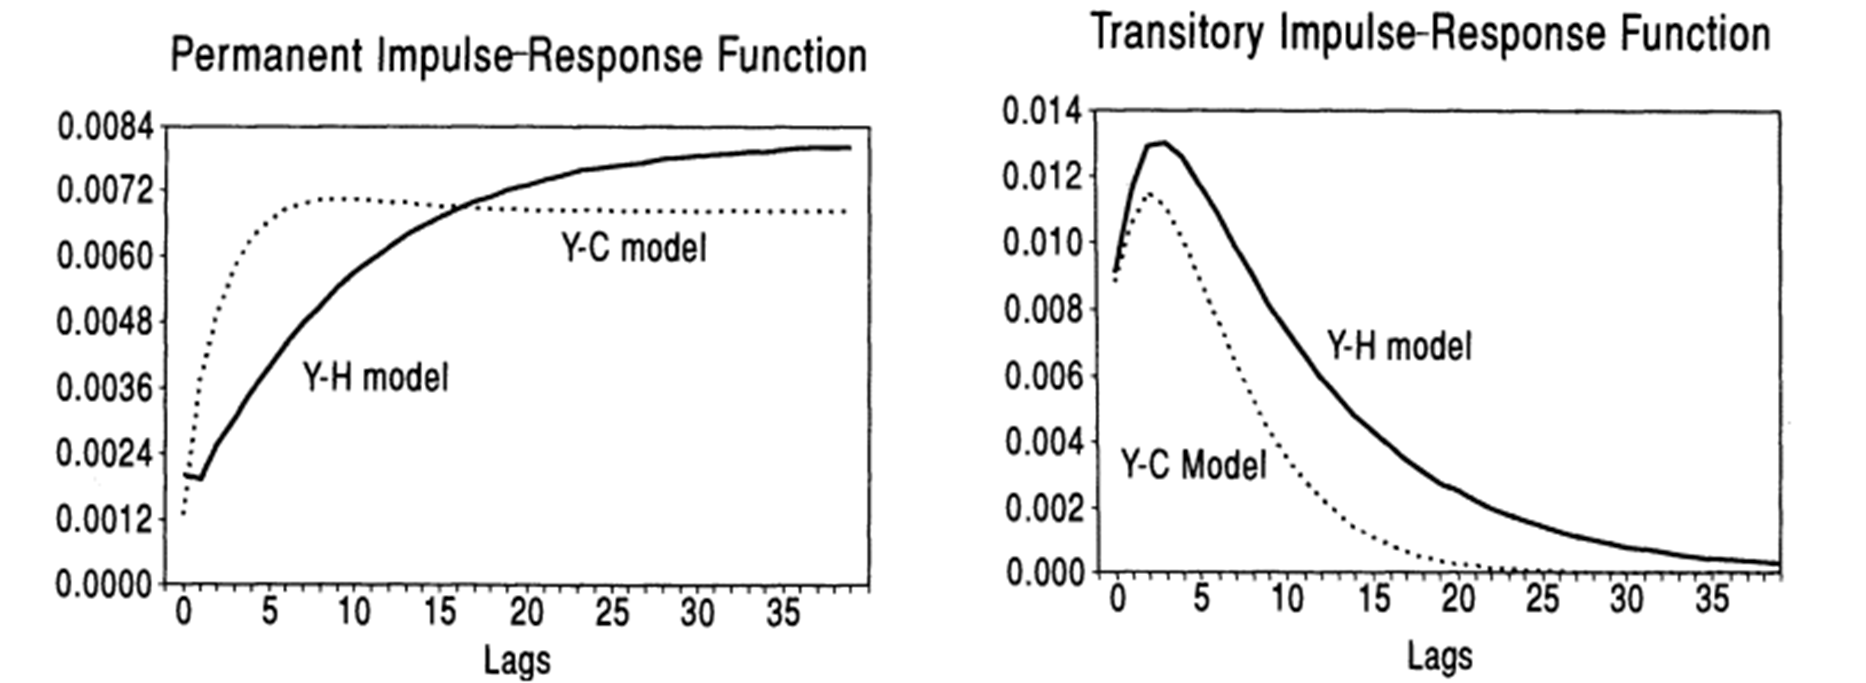
\includegraphics[width=10cm]{sf2.png}
        \caption{Impulse-response functions for output growth}
    \end{figure}
\end{frame}

\begin{frame}
    \begin{itemize}
    \setlength\itemsep{1em}
        \item \alert{Theoretical} part: 3 models
        \begin{enumerate}
            \item Baseline RBC
            \item Baseline RBC + capital adjustment cost
            \item Baseline RBC + labor adjusment cost
        \end{enumerate}
        \item Models examination:
            \begin{itemize}
                \item For each model: Simulate shocks $\Rightarrow$ 1,000 \alert{Monte-Carlo simulations} 
                \item Estimate autocorrelation and IRF for each artificial sample
                \item[$\Rightarrow$] Compute \alert{probability of observing the stylized facts} in generated data
            \end{itemize}
    \end{itemize}
\end{frame}

\begin{frame}{Baseline RBC (how many times I have seen you...)}
Representative agent: 

    
\end{frame}
%\begin{frame}{Introduction}
%    It establishes a link between the \alert{theoretical} RBC model literature and the \alert{empirical} output dynamics analysis.
%    \begin{itemize}
%        \item Theoretical (3 models): 
%        \begin{enumerate}
%            \item Baseline RBC
%            \item Baseline + capital adjustment cost
%            \item Baseline + labor adjustment cost
%        \end{enumerate}
%        \item Empirical (4 graphs)
%        \begin{enumerate}
%            \item output growth $\Delta y_t$ behavior: autocorrelation function \& spectrum decomposition
%            \item impulse response: to \alert{permanent} shock $\varepsilon_z$ \& \alert{temporary} shock $\varepsilon_g$
%        \end{enumerate} 
%    \end{itemize}
%They calibrate the model with real world data $\to$ simulate shocks to feed into the model $\to$ graph and %compare the simulated responses with that of empirical observations.
%
%    \note[itemize]{
%    \item point 1
%    \item point 2
%    }
%\end{frame}

\begin{frame}{Focus (all about shocks...)}
\metroset{block=fill}
        \begin{exampleblock}{Theory}
            Propagation mechanisms embedded in the model resulted in different $\Delta y_t$ responses to shocks $\varepsilon_z$ and $\varepsilon_g$ 
        \end{exampleblock}
        \begin{align}
            &(1-L) \ln \left(a_{t}\right)=\mu+\varepsilon_{\mathrm{a} t} \\
            &\ln \left(g_{t}\right)-\ln \left(a_{t}\right)=\bar{g}+\varepsilon_{g t} /(1-\rho L) 
        \end{align}
     
        \begin{exampleblock}{Empirical}
        An important component in empirical analysis is how to identify $\varepsilon_z$ and $\varepsilon_g$ from observation of $\Delta y_t$.
    \end{exampleblock}
\end{frame}


\section{Main Idea}
\subsection{Baseline Model}

\begin{frame}{Estimation and Simulation}
    \begin{itemize}
        \item Estimation
            \begin{itemize}
                \item Christiano and Eichenbaum (1992) estimate, $\mu = 0.004, \bar{g} = 0.177$, and $p = 0.96$
                \item Rescale the innovation variances to match the sample variance of per capita GNP growth: $\sigma_a = 0.0097$ and $\sigma_g = 0.0113$
            \end{itemize}
        \item Monte Carlo Simulation
            \begin{itemize}
                \item Generate artificial data over a time horizon of 140 quarters to match the length of sample period
                \item Each model was simulated 1,000 times
                \item Autocorrelation and impulse-response functions were estimated for each artificial sample
            \end{itemize}
        
    \end{itemize}
\end{frame}


\begin{frame}{Baseline model simulation and comparison}
\begin{figure}
    \centering
  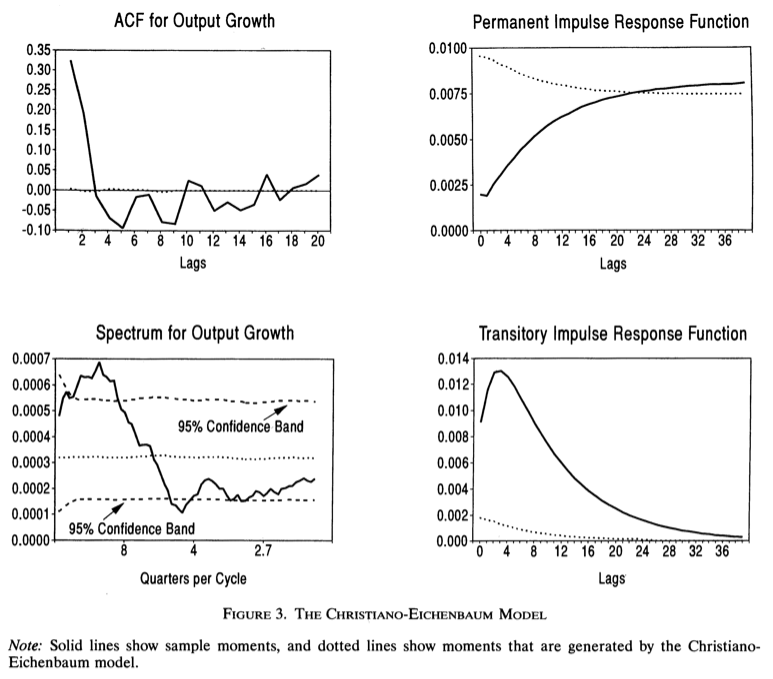
\includegraphics[width=0.57\linewidth]{baseline_all.png}
  %\caption{}
\end{figure}
\small
\begin{itemize}
    \item  ACF are close to zero $\Rightarrow$  No serial correlation
    \item Spectrum is quite flat $\Rightarrow$ No Business-cycle periodicity in output growth
    \item Some success matching the permanent IRF
    \item The model strongly damps transitory shock and generates monotonic decay $\Rightarrow$ No trend-reverting component in output
\end{itemize}
\end{frame}

\subsection{Gestation Lags and Capital Adjustment Costs}

\begin{frame}{Gestation Lags and Capital Adjustment Costs}

\begin{itemize}
    \item \textbf{Time-to-build Model}
    
    Firms face a 3-quarter gestation lag when installing new capital

    \item \textbf{Q-theoretic Model}
   
    Quadratic costs of adjusting the capital stocks

    Production function becomes:
    $$
\ln \left(y_t\right)= \ln \left[f\left(k_t, a_t n_t\right)\right] -\left(\alpha_{k} / 2\right)\left[\Delta k_t / k_{t-1}\right]^2
$$

Based on Shapiro (1986), $\alpha_{k}$ is calibrated to be 2.2
\end{itemize}

\end{frame}

\begin{frame}{Comparison}
\begin{figure}
    \centering
  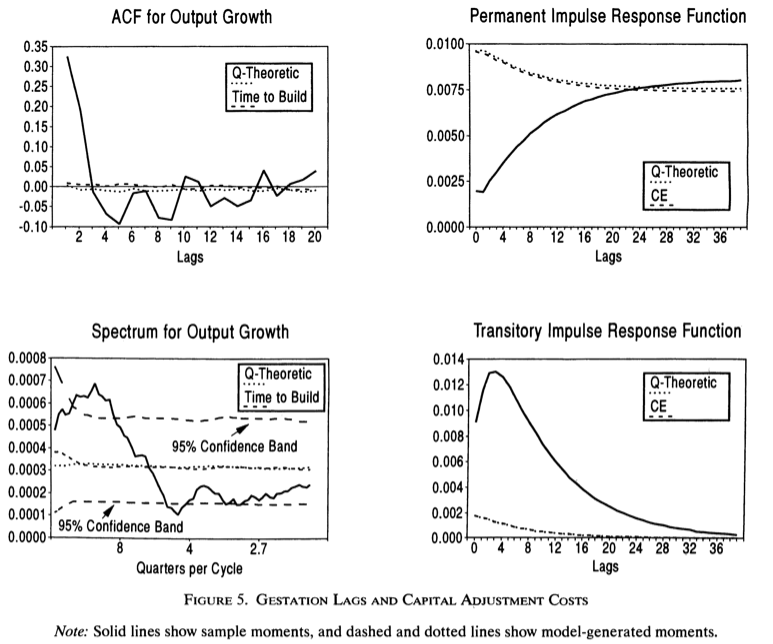
\includegraphics[width=0.65\linewidth]{Capital adj cost.png}
  %\caption{}
\end{figure}
\small
\begin{itemize}
    \item No serial correlation or Business-cycle periodicity in output growth
    \item No effect on IRF $\Rightarrow$ No help to propagate shocks
    \begin{itemize}
        \item Gestation Lags and Capital Adjustment Costs alter $I_t$, but $I_t$ is small relative to $k_t$ $\Rightarrow$ little effect on $y_t$
    \end{itemize}
\end{itemize}
    
\end{frame}

\subsection{Employment Lags and Labor Adjustment Costs}
\begin{frame}{Employment Lags and Labor Adjustment Costs}
\begin{itemize}
    \item \textbf{Adjustment-cost model}

Production function:
$$
\ln \left(y_t\right)= \ln \left[f\left(k_t, a_t n_t\right)\right] -\left(\alpha_{k} / 2\right)\left[\Delta k_t / k_{t-1}\right]^2 -\left(\alpha_n / 2\right)\left[\Delta n_t / n_{t-1}\right]^2
$$

Shapiro's estimate : $\alpha_{k} = 0.36$

    \item \textbf{Labor-hoarding model} Burnside et al. (1993)

    Firms must choose the size of the labor force before observing the current state of the economy but can vary the intensity of work effort after observing the current state
\end{itemize}


\end{frame}

\begin{frame}{Comparison}
\begin{figure}
    \centering
  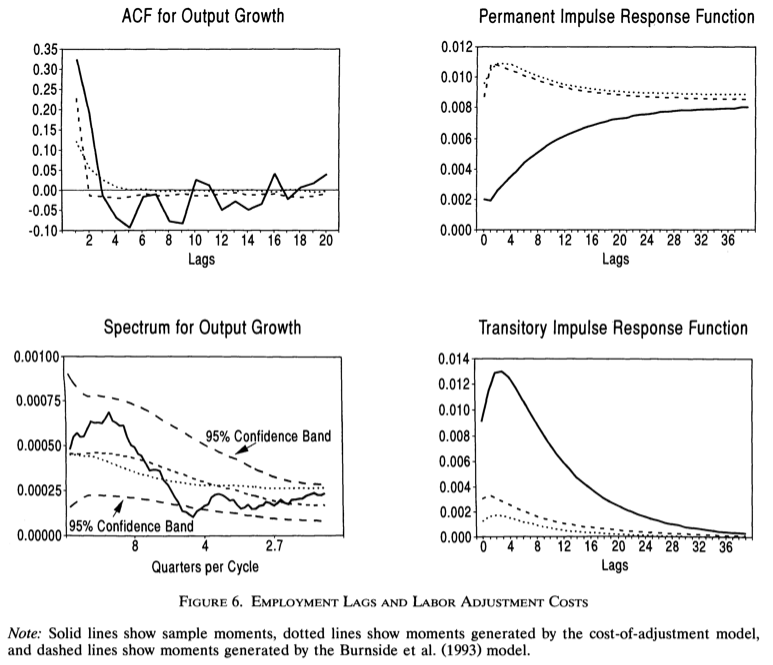
\includegraphics[width=0.57\linewidth]{labor cost.png}
  %\caption{}
\end{figure}
{\footnotesize
\begin{itemize}
    \item Positive autocorrelation at lag 1, and modest negative autocorrelation at higher-order lags in output growth
    % \begin{itemize}
    %     \item Burnside et al. (1993) model: positively autocorrelated at lag 1 and has modest negative autocorrelation at higher-order lags
    %     \item Adjustment-cost model: output growth is well approximated by an AR(1), with positive autocorrelation at lag 1 and monotonic decay at higher-order lags
    % \end{itemize}
    \item Modest business-cycle periodicity
    \item Overstate the short-term response of permanent shocks and understate its response to transitory shock
    \item No important trend-reverting component in output
\end{itemize}}
\end{frame}

\section{Contribution}

\begin{frame}{Contribution}
\begin{itemize}
    \item Baseline model and gestation lags and capital adjustment costs model have weak internal propagation mechanisms and do not generate dynamics via their internal structure
    \item Models that rely on lags or costs of adjusting labor input are partially successful: 
    \begin{itemize}
        \item Right pattern of autocorrelation in output growth
        \item Small hump in transitory IRF
    \end{itemize}
\end{itemize}
    
\end{frame}

\begin{frame}{ACF for Output Growth} 
\begin{minipage}{0.33\textwidth}
\begin{figure}
  \centering
  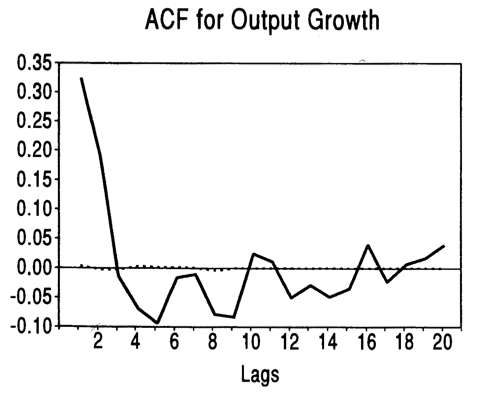
\includegraphics[width=\linewidth]{Bse_ACF.png}
  \caption{Baseline Model}
\end{figure}
\end{minipage}%
\begin{minipage}{0.33\textwidth}
\begin{figure}
  \centering
  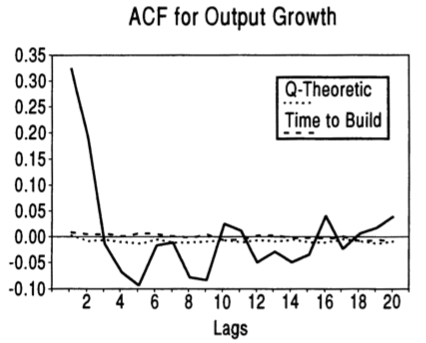
\includegraphics[width=\linewidth]{K_ACF.png}
  \caption{Capital Adjustment Cost}
\end{figure}
\end{minipage}%
\begin{minipage}{0.33\textwidth}
\begin{figure}
  \centering
  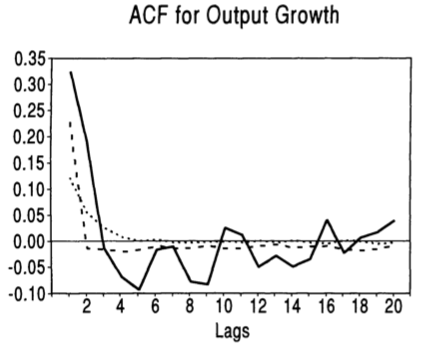
\includegraphics[width=\linewidth]{L_ACF.png}
  \caption{Labor Adjustment Cost}
\end{figure}
\end{minipage}

\begin{itemize}
    \item Baseline \& Capital: No serial autocorrelation
    \item Labor: Positive autocorrelation at lag 1
\end{itemize}

\end{frame}


\begin{frame}{Spectrum for Output Growth}  
\begin{minipage}{0.33\textwidth}
\begin{figure}
  \centering
  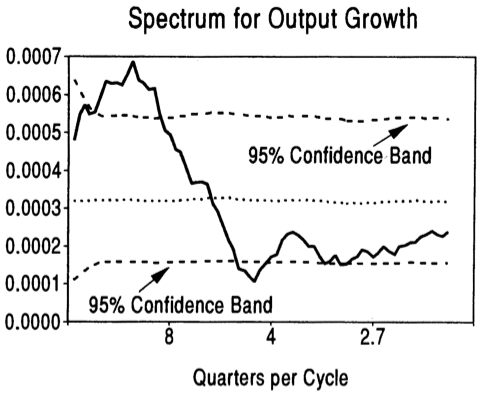
\includegraphics[width=\linewidth]{Base_spect.png}
  \caption{Baseline Model}
\end{figure}
\end{minipage}%
\begin{minipage}{0.33\textwidth}
\begin{figure}
  \centering
  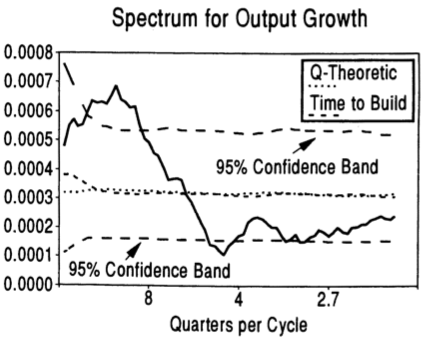
\includegraphics[width=\linewidth]{K_spect.png}
  \caption{Capital Adjustment Cost}
\end{figure}
\end{minipage}%
\begin{minipage}{0.33\textwidth}
\begin{figure}
  \centering
  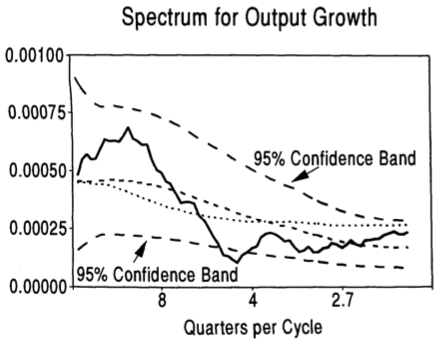
\includegraphics[width=\linewidth]{L_spect.png}
  \caption{Labor Adjustment Cost}
\end{figure}
\end{minipage}

\begin{itemize}
    \item Baseline \& Capital: Spectrum is quite flat $\Rightarrow$ No Business-cycle periodicity in output growth
    \item Labor: Modest business-cycle periodicity
\end{itemize}

\end{frame}

\begin{frame}{Permanent Impulse Response Function} 
\begin{minipage}{0.33\textwidth}
\begin{figure}
  \centering
  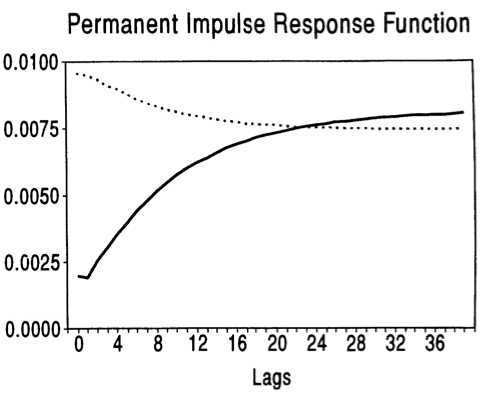
\includegraphics[width=\linewidth]{Base_per_IRF.png}
  \caption{Baseline Model}
\end{figure}
\end{minipage}%
\begin{minipage}{0.33\textwidth}
\begin{figure}
  \centering
  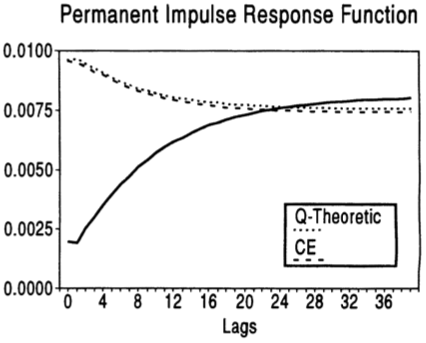
\includegraphics[width=\linewidth]{K_per_IRF.png}
  \caption{Capital Adjustment Cost}
\end{figure}
\end{minipage}%
\begin{minipage}{0.33\textwidth}
\begin{figure}
  \centering
  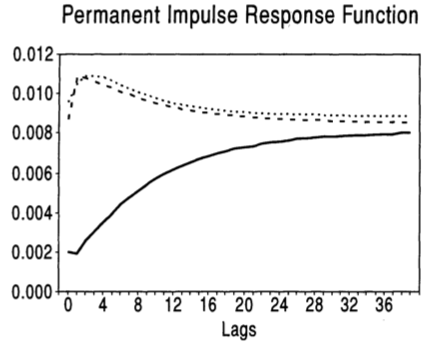
\includegraphics[width=\linewidth]{L_per_IRF.png}
  \caption{Labor Adjustment Cost}
\end{figure}
\end{minipage}

\begin{itemize}
    \item Baseline \& Capital: Some success in matching the permanent IRF
    \item Labor: Hump-shared response of output to technology shocks
\end{itemize}

\end{frame}

\begin{frame}{Transitory Impulse Response Function}  
\begin{minipage}{0.33\textwidth}
\begin{figure}
  \centering
  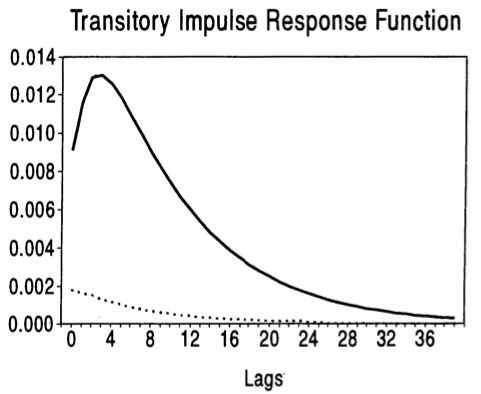
\includegraphics[width=\linewidth]{Base_trans_IRF.png}
  \caption{Baseline Model}
\end{figure}
\end{minipage}%
\begin{minipage}{0.33\textwidth}
\begin{figure}
  \centering
  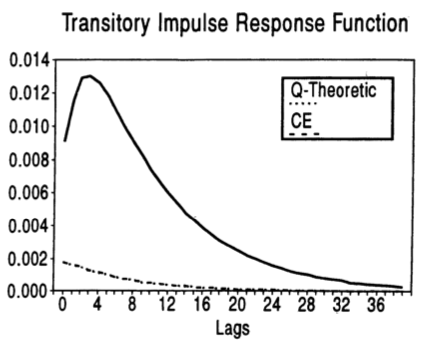
\includegraphics[width=\linewidth]{K_trans_IRF.png}
  \caption{Capital Adjustment Cost}
\end{figure}
\end{minipage}%
\begin{minipage}{0.33\textwidth}
\begin{figure}
  \centering
  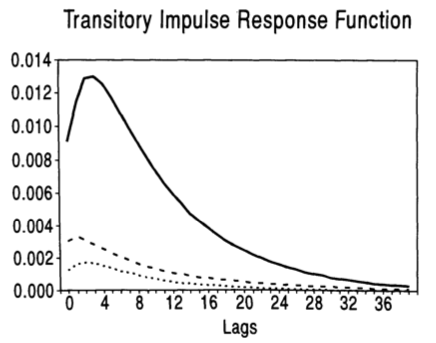
\includegraphics[width=\linewidth]{L_trans_IRF.png}
  \caption{Labor Adjustment Cost}
\end{figure}
\end{minipage}
\begin{itemize}
    \item Baseline \& Capital: Wrong qualitative and quantitative response to transitory shocks
    \item Labor: Right qualitative response to transitory shocks, but too small in magnitude
\end{itemize}

\end{frame}


\end{document}
